% unified_sindy.tex
% See accompanying readme.txt for copyright statement, change log etc.

% Any modification of this template, including writing a paper using it,
% MUST rename the file i.e. use a different file name.

%%%%%%%%%%%%%%%% START OF PREAMBLE %%%%%%%%%%%%%%%

% Basic setup. Authors shouldn't need to adjust these commands.
% It's annoying, but please do NOT strip these into a separate file.
% They need to be included in this .tex for our production software to work.

% Use the basic LaTeX article class, 12pt text
\documentclass[12pt]{article}

% Science uses Times font. If you don't have this installed (most LaTeX installations will be
% fine) or prefer the old Computer Modern fonts, comment out the following line
\usepackage{newtxtext,newtxmath}
% Depending on your LaTeX fonts installation, you might get better results with one or both of these:
%\usepackage{mathptmx}
%\usepackage{txfonts}

% Allow external graphics files
\usepackage{graphicx}

% Use US letter sized paper with 1 inch margins
\usepackage[letterpaper,margin=1in]{geometry}

% Double line spacing, including in captions
\linespread{1.5} % For some reason double spacing is 1.5, not 2.0!

% One space after each sentence
\frenchspacing

% Abstract formatting and spacing - no heading
\renewenvironment{abstract}
	{\quotation}
	{\endquotation}

% No date in the title section
\date{}

% Reference section heading
\renewcommand\refname{References and Notes}

% Figure and Table labels in bold
\makeatletter
\renewcommand{\fnum@figure}{\textbf{Figure \thefigure}}
\renewcommand{\fnum@table}{\textbf{Table \thetable}}
\makeatother

% Call the accompanying scicite.sty package.
% This formats citation numbers in Science style.
\usepackage{scicite}

% Provides the \url command, and fixes a crash if URLs or DOIs contain underscores
\usepackage{url}

%%%%%%%%%%%% CUSTOM COMMANDS AND PACKAGES %%%%%%%%%%%%

% Authors can define simple custom commands e.g. as shortcuts to save on typing
% Use \newcommand (not \def) to avoid overwriting existing commands.
% Keep them as simple as possible and note the warning in the text below.
% Example:
\newcommand{\pcc}{\,cm$^{-3}$}	% per cm-cubed

% Please DO NOT import additional external packages or .sty files.
% Those are unlikely to work with our conversion software and will cause problems later.
% Don't add any more \usepackage{} commands.


%%%%%%%%%%%%%%%% TITLE AND AUTHORS %%%%%%%%%%%%%%%%

% Title of the paper.
% Keep it short and understandable by any reader of Science.
% Avoid acronyms or jargon. Use sentence case.
\def\scititle{
	Unified Implicit and Exlicit Sparse Identification of NonLinear Dynamical Systems for Lagrangian and Newtonian catalogs.
}
% Store the title in a variable for reuse in the supplement (otherwise \maketitle deletes it)
\title{\bfseries \boldmath \scititle}

% Author and institution list.
% Institution numbers etc. should be hard-coded, do *not* use the \footnote command.
\author{
	% You can write out first names or use initials - either way is acceptable, but be consistent
	Eymeric~Chauchat$^{1\ast}$,
	Mitsuhiro~Hayashibe$^{1}$\and
	%Someone~E.~Else$^{2}$\and
	% Additional lines of authors should be inserted using the \and command (not \\)
	% Institution list, in a slightly smaller font
	\small$^{1}$Department of Robotics, Tohoku University, Sendai, Miyagi 980-8577, Japan.\and
	%\small$^{2}$Another Department, Different Institution, City \& Postal Code, Country.\and
	% Identify at least one corresponding author, with contact email address
	\small$^\ast$Corresponding author. Email: chauchat.eymeric.r7@dc.tohoku.ac.jp%\and
	% Joint contributions can be indicated like this
	%\small$^\dagger$These authors contributed equally to this work.
}

%%%%%%%%%%%%%%%%% END OF PREAMBLE %%%%%%%%%%%%%%%%


%%%%%%%%%%%%%%%% START OF MAIN TEXT %%%%%%%%%%%%%%%
\begin{document} 

% Insert the title and author list
\maketitle

% Abstract, in bold
% There are strict length limits, and not all formats have abstracts.
% Consult the journal instructions to authors for details.
% Do not cite any references in the abstract.
\begin{abstract} \bfseries \boldmath
% Start with one or two sentences of background
This is a simple template to prepare papers in \LaTeX\ for the \textit{Science}-family journals.
Abstracts start with one or two sentences of background, which should be
comprehensible to any scientist.
% Then summarise the results of your observations, experiments, simulations etc.
The following text should outline the main results of the research.
Simple mathematical expressions can be included e.g. $a^2+b^2=c^2$.
% End with a statement of your main conclusions
The final sentence of the abstract should state the main conclusions and implications.
\end{abstract}


% The first paragraph of any Science paper does NOT have a heading
% Nor is it indented
% \noindent
% The main text should begin with a brief introduction to the topic, at a level which is understandable by
% scientists in adjacent disciplines. Provide enough information to put your work in context,
% but do not attempt a comprehensive review.

% General guidance on \LaTeX:
% The \textit{Science}-family journals accept papers written in \LaTeX, but they are a minority
% of the submissions we receive. Our production department does not handle \LaTeX\ directly,
% instead we use conversion software to automatically process the .tex file into a format they
% can use. That works well \textit{provided the .tex file is straightforward}. Keep it simple
% and follow this template. Don't import additional packages or define complex new commands.

% Figures and tables:
% These should be inserted at the end of the main text, as below (not in the middle of the text).
% Refer to them using e.g.~Figure~\ref{fig:example} (or Fig.~\ref{fig:example}) and Table~\ref{tab:example}.

% Citing references:
% Science uses a numeric citation system. Cite references by number e.g.~\cite{example}.
% The template will combine reference numbers automatically~\cite{example,example2},
% including ranges~\cite{example,example2, example_preprint}.
% Reference author names and years should be stated in the reference list, not in the text.
% If you want to add a comment, use the syntax [see \cite{example} for details].
% Not \cite[see][for details]{example}. Unfortunately that isn't compatible with scicite.sty

% Referring to supplementary material:
% Whenever more details are given in the Materials and Methods section, cite an entry in
% the reference list that directs readers there, like this~\cite{methods}.
% To refer to material in the Supplementary Text section, just write (Supplementary Text).
% See guidance below for the difference between those two types of supplementary material.
% Supplementary figures and tables are referred to in lowercase
% e.g.~figure~\ref{fig:sup_example} or table~\ref{tab:sup_example}.
% Material in separate files needs to be hand coded e.g.~data~S1, movie~S2.

% Mathematics:
% Simple mathematical expressions can be inserted in the text like $2\times3=6$.
% Variables should be italic but textual labels are roman e.g.~$T_\text{max}$.
% Explain the meaning of all variables on their first appearance.
% More complicated expressions should be entered as numbered equations, such as

% \begin{equation}
% 	x=\frac{-b\pm\sqrt{b^2-4ac}}{2a}.
% 	\label{eq:example} % Use a logical label
% \end{equation}

% \noindent\ Do not indent text immediately after an equation.
% They can be referred back to as e.g.~Equation~\ref{eq:example}.

% Formatting:
% Names of software packages should be set in small capitals e.g.~\textsc{NumPy}.
% Use a non-breaking space between a number and its unit e.g.~7.4~km,
% and thin spaces between different parts of a unit e.g.~12~m\,s$^{-1}$.
% Use $\pm$ (not parentheses) to indicate uncertainties e.g.~$g=9.8\pm0.2$~m\,s$^{-2}$.

% Research Articles and Reviews split the text into sections using headings
% Use a short (up 6 words) descriptive phrase, not generic 'Results' or 'Conclusions'
% Most other formats do not have headings, see the journal instructions to authors for details
% \subsection*{An example heading}
% Research Articles and Reviews use headings to split the main text into sections;
% most other formats do not have headings.

% Length limits:
% The \textit{Science}-family journals impose limits on the number of words, figures\slash
% tables, and references cited in the main text.
% The limits vary between the journals and article types.
% Refer to the instructions to authors on the journal website for the current limits.


% If your text is very short you might need to uncomment the following line to avoid
% layout problems with the figures and tables.
%\newpage

\subsection*{Result}

\subsubsection*{New Unified SINDy catalog and experiment matrix}

We consider a mechanical system of $n$ generalised-coordinate $\mathbf{q}=(q_i)_{i=1}^n$, which conservative dynamics can be determined by a lagrangian $\mathcal{L}$ and a set of non-conservative forces $(Q^{nc}_i)_{i=1}^n$ for each coordinate. The system is also externally excited by forces $(Q^{ext})_{i=1}^n$. Following Euler-lagrange the dynamics of our system can be written as a system of equation for each $i$ in $n$:

\begin{equation}
	Q^{ext}_i + Q^{nc}_i  = \frac{d}{dt}\left( \frac{\partial \mathcal{L}}{\partial \dot{q}_i}\right) - \frac{\partial \mathcal{L}}{\partial q_i} 
	\label{eq:initial-dynamics}
\end{equation}

If we assume that the lagrangian $\mathcal{L}$ expression is a linear combination of non linear candidate function :

\begin{equation}
	\mathcal{L} = \sum_{k=1}^{m} c_k \xi_k(\mathbf{q},\dot{\mathbf{q}})
\end{equation}

and that each of the non-conservative force is a linear combination of non linear candidate function independant of the coordinate\footnote{coefficient is null on canditate function that are not present on other coordinate} :

\begin{equation}
	Q^{nc}_i = \sum_{k=1}^{p} b^i_k \phi_k(\mathbf{q},\dot{\mathbf{q}},\ddot{\mathbf{q}})
\end{equation}

Thanks to the linearity of euler lagrange equation we can rewrite the initial system dynamics Eq.~\ref{eq:initial-dynamics} in the following form for each of the coordinate:

\begin{equation}
	\sum_{k=1}^{n} \delta_{ik} Q^{ext}_k + \sum_{k=1}^{p} b^i_k \phi_k  = \sum_{k=1}^{m} c_k \left( \frac{d}{dt}\left( \frac{\partial \xi_k}{\partial \dot{q}_i}\right) - \frac{\partial \xi_k}{\partial q_i} \right) 
	\label{eq:UNI-system}
\end{equation}

By flattening the coefficient $(b^i_k)_{1 \le i \le n, \, 1 \le k \le p}$, we can obtain a classical SINDy coefficient vector :

\begin{equation}
	\Xi = \left[1,\dots,1 ,b^1_1,\dots,b^n_1,\dots,b^n_p,c_1,\dots,c_m\right]
\end{equation}
\noindent where $n$ successive $1$ are placed at the begining in order to account for the $Q^{ext}$ external forces term in our catalog. 

In the mean time we obtain the experiment matrix Fig.~\ref{fig:uni-sindy-matrix} that match our cofficient vector $\Xi$.

\subsection*{Result}

Detailed explanation on data generation and regression mode are in \cite{methods}.

The goal of the experiments we conducted is to show that UNI-SINDy get on par result with former SINDy method in each of their respective performance area, and also show that UNI-SINDy outperform old method on mixed passive active system. This latter kind of system ressemble more real robot that have passive part (typically in soft or under-actuaded robot) and active part.

We have divided the experiments in different group, in order to explicity compare UNI-SINDy in different area :
\begin{itemize}
	\item \textbf{No damping explicit forces :} compare XL-SINdy with the new framework
	\item \textbf{Any damping explicit forces :} compare SINDy with the new framework
	\item \textbf{Any damping no forces :} compare SINDy-PI with the new framework
	\item \textbf{Any damping mixed implicit explicit forces : } show the versatility of the new UNI-SINDy when dealing with new type of experiment
\end{itemize}

Following the \textbf{data generation and processing part} of \cite{methods}

\newpage

%%%%%%%%%%%%%%%% MAIN TEXT FIGURES %%%%%%%%%%%%%%%

\begin{figure} % Do NOT use \begin{figure*}
	\centering
	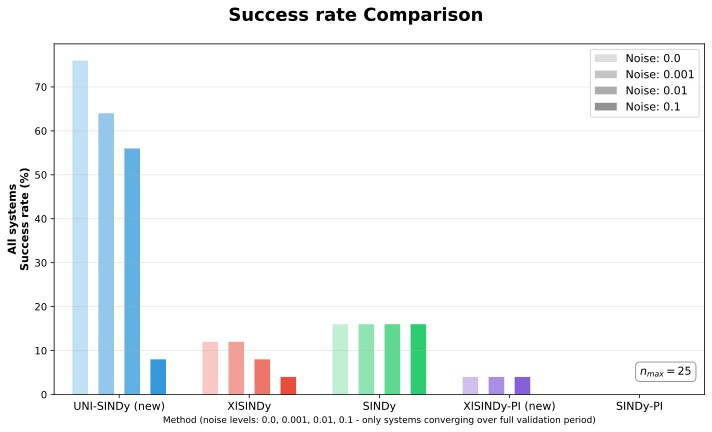
\includegraphics[width=0.6\textwidth]{success_rate_combined_white_background} % for an image file named example_figure.*
	% Pick an appropriate width - in print, figures are usually one or two columns wide, which can
	% be approximated by 0.3\textwidth or 0.6\textwidth respectively. Use appropriate label sizes.

	% Captions go below figures
	\caption{\textbf{Success rate of each method over different noise level.}
		Every algorithm has been presented with same training data gathered over 192 different base experiment. On these 192 experiments only 65 have got at least one algorithm successful. On these 65 experiments we have plotted the success rate on each of this experiments for every noise level and every algorithm. }
	\label{fig:example} % give each figure a logical label name
\end{figure}


%%%%%%%%%%%%%%%% MAIN TEXT TABLES %%%%%%%%%%%%%%%

% \begin{table} % Do NOT use \begin{table*}
% 	\centering
% 	% Captions go above tables
% 	\caption{\textbf{All captions must start with a short bold sentence, acting as a title.}
% 		Then explain what is being listed in the table, the meaning of each column etc.
% 		Captions are placed above tables.}
% 	\label{tab:example} % give each table a logical label name
	
% 	\begin{tabular}{lccc} % four columns, alignment for each
% 		\\
% 		\hline
% 		Sample & $A$ & $B$ & $C$\\
% 		 & (unit) & (unit) & (unit)\\
% 		\hline
% 		First & 1 & 2 & 3\\
% 		Second & 4 & 6 & 8\\
% 		Third & 5 & 7 & 9\\
% 		\hline
% 	\end{tabular}
% \end{table}



%%%%%%%%%%%%%%%% REFERENCES %%%%%%%%%%%%%%%

\clearpage % Clear all remaining figures and tables then start a new page

% The list of references goes after the main text and before the acknowledgements
% When preparing an initial submission, we recommend you use BibTeX, like this:
%
\bibliography{unified_sindy} % for a file named science_template.bib
\bibliographystyle{sciencemag}

% After the paper has completed peer review and been revised ready for acceptance,
% you should comment out the lines above and copy-paste the contents of your .bbl
% file here instead. This will help ensure that our conversion software works correctly.
% Remember to re-run BibTeX first - check the timestamp!
%
% Example of the first three entries copy-pasted from science_template.bbl:
%
%\begin{thebibliography}{1}
%
%\bibitem{example}
%A.~N. {Author}, An example reference. \emph{Journal of Improbable Research}
%  \textbf{1}, 67 (2020).
%
%\bibitem{example2}
%F.~M. {Surname}, S.~{Author}, A second example. \emph{Interesting Research
%  Letters} \textbf{32}, 897 (2019).
%
%\bibitem{example_preprint}
%P.~{One}, P.~{Two}, P.~{Three}, {An unpublished preprint}. \emph{preprint}
%  (2021), arXiv:2101.12345.
%
%\end{thebibliography}


%%%%%%%%%%%%%%%% ACKNOWLEDGEMENTS %%%%%%%%%%%%%%%

% \section*{Acknowledgments}
% Here you can thank helpful colleagues who did not meet the journal's authorship criteria, or
% provide other acknowledgements that don't fit the (compulsory) subheadings below.
% Formatting requirements for each of these sections differ between the \textit{Science}-family
% journals; consult the instructions to authors on the journal website for full details.
% \paragraph*{Funding:}
% List the grants, fellowships etc. that funded the research;
% use initials to specify which author(s) were supported by each source.
% Include grant numbers when appropriate or required by the funding agency.
% For example: F.~A. was funded by the Generous Science Agency grant~2372.
\paragraph*{Author contributions:}
E.C : \textsc{py-xl-sindy} developper and manuscript writter
% \paragraph*{Competing interests:}
% Disclose any potential conflicts of interest for all authors, such as patent applications,
% additional affiliations, consultancies, financial relationships etc.
% See the journal editorial policies web page for types of competing interest that must be declared.
% If there are no competing interests, state:
% ``There are no competing interests to declare.''
\paragraph*{Data and materials availability:}

Every subsequent material is disclosed with MIT licence. 
\begin{itemize}
\item \textsc{py-xl-sindy} : {\tiny\url{https://github.com/Eymeric65/py-xl-sindy}}, main library containing the code source in order to use the new Unified SINDy algorithm. Contains also new implementation of SINDy, SINDy-PI and Xl-SINDy
\item \textsc{py-xl-sindy-data-visualisation} : {\tiny\url{https://github.com/Eymeric65/py-xl-sindy-data-visualisation}}, additionnal library containing data generation script, batch processing data, paper, figures, presentation slide and visualisation website source code.
\item {\tiny\url{https://eymeric65.github.io/py-xl-sindy-data-visualisation/}} : visualisation website of every trajectory generated with every result used for plotting the different summary graph from the paper
\end{itemize}
% Specify where the data, software, physical samples, simulation outputs or other materials
% underlying the paper are archived.
% They must be publicly accessible when the paper is published (without embargo) and enable
% readers to reproduce all the results in the paper.
% Contact the editor if you’re unsure what needs to be shared.

% Our preference is for digital material to be deposited in a suitable non-profit online data or
% software repository that issues the material with a DOI.
% Alternatively, an institutional repository, subject-based archive, commercial repository etc.
% is acceptable, as are (short) supplementary tables or a machine-readable supplementary data file.
% ‘Available on request’ or personal web pages are not allowed.

% Cite the relevant DOI \cite{dataset}, URL \cite{example_url} or reference \cite{example2}
% in this statement.
% These \textit{do not} count towards the reference limit if they are only cited in the acknowledgements.
% Be specific and state a unique identifier -- such as an accession number, software version number
% or observation ID -- so readers can easily retrieve the exact material used.

% Declare any restrictions on sharing or re-use -- such as a Materials Transfer Agreement (MTA) or
% legal restrictions -- which must be approved by your editor.
% Unreasonable restrictions will preclude publication.
% Consult the journal's editorial policies web page for more details.


%%%%%%%%%%%%%%%% SUPPLEMENT LIST %%%%%%%%%%%%%%%

% List the contents of your Supplementary Materials, including the numbers of any
% supplementary figures, tables, external data files etc. and any references that are
% cited only in the supplement. In this example, refs. 7-8 are cited only in the supplement.
% Fill out your numbers accordingly and delete any lines that aren't applicable.
\subsection*{Supplementary materials}
Materials and Methods\\
Supplementary Text\\
Figs. S1 to S3\\
Tables S1 to S4\\
References \textit{(7-\arabic{enumiv})}\\ % automatically fills out the last reference number
% (filling out the other numbers automatically is possible but fiddly and liable to break)
Movie S1\\
Data S1

%%%%%%%%%%%%%%%% END OF MAIN TEXT %%%%%%%%%%%%%%%

\newpage

%%%%%%%%%%%%%%%% START OF SUPPLEMENT %%%%%%%%%%%%%%%

% Figures, tables, equations and pages in the supplement are numbered S1, S2 etc.
\renewcommand{\thefigure}{S\arabic{figure}}
\renewcommand{\thetable}{S\arabic{table}}
\renewcommand{\theequation}{S\arabic{equation}}
\renewcommand{\thepage}{S\arabic{page}}
\setcounter{figure}{0}
\setcounter{table}{0}
\setcounter{equation}{0}
\setcounter{page}{1} % not 0 as \newpage already started a supplementary page
% References continue the numbering from the main text.


%%%%%%%%%%%%%%%% SUPPLEMENT TITLE PAGE %%%%%%%%%%%%%%%

\begin{center}
\section*{Supplementary Materials for\\ \scititle}

% Author list for the supplement
% Indicate the corresponding authors, but do NOT include institutions here
% It would be nice if the template auto-generated this, but doing so is complicated...
Eymeric~Chauchat$^{\ast}$,
Mitsuhiro~Hayashibe\\ % we're not in a \author{} environment this time, so use \\ for a new line
\small$^\ast$Corresponding author. Email: chauchat.eymeric.r7@dc.tohoku.ac.jp\\
\end{center}

% Fill out the numbers for each type of supplementary material,
% and delete any lines that aren't applicable.
% These are just example numbers that don't match the rest of this template.
\subsubsection*{This PDF file includes:}
Materials and Methods\\
Supplementary Text\\
Figures S1 to S3\\
Tables S1 to S4\\
Captions for Movies S1 to S2\\
Captions for Data S1 to S2

\subsubsection*{Other Supplementary Materials for this manuscript:}
Movies S1 to S2\\
Data S1 to S2

\newpage

%%%%%%%%%%%%%%%% MATERIALS AND METHODS %%%%%%%%%%%%%%%

\subsection*{Materials and Methods}

We introduce two new mechanisms onto the standard SINDy \cite{bruntonDiscoveringGoverningEquations2016} algorithm. The first one is the unified catalog. As explained in the introduction SINDy result are highly dependant on the quality of the catalog provided. While specialised catalog like Lagrange may fulfill highly specialised case study, it fails when faced with phenomenum it can not represent. The opposite is also true when using Newtonian catalogs, the general reach of the catalog enable the discovery of every type of dynamics but at the cost of large catalog that become a computational burden. Newton and Lagrange are however linked by the Euler-Lagrange equation, by leveraging this equation we were able to create a new unified experiment matrix where both paradigm are cooperating Figure.~\ref{fig:uni-sindy-matrix}. This can be futhermore extended to any paradigm that have such a translation equation. By using this new unified catalog and experiment matrix we are able to grasp a larger variety of dynamics while keeping the catalog size low.

The second mechanism that we introduce is the mixed implicit-explicit solving. From past studies we could execute system identification in explicit and implicit case separately, however when dealing with multiple coordinate system the nature of the system becomes ambiguous. We can ask ourself what is the implicit and explicit part in a system where we have input forces only on a subset of coordinates (a system composed of active and passive joint). We have thus developped an algorithm in order to determine during the regression process what could be the implicit and explicit part of the system. The algorithm is described in Figure.~\ref{fig:mixed_algorithm}.

\subsubsection*{Data generation and processing}

Our goal is to compare the performance of the new unified implicit-explit multi paradigm SINDy with the past Xl-SINDy, SINDy and SINDy-PI algorithms. We have compared these algorithms on three different systems: cartpole, cartpole double (double pendulum on a cartpole) and double pendulum. We have generated trajectory on these systems using a random harmonic input forces (sum of harmonic functions with random frequencies and amplitudes) that can be applied on every joint (fully explicit), on a subset of joints (mixed implicit-explicit) or no joint at all (implicit). In order to guarantee fair comparison between paradigm, we have guaranteed that input knowledge put inside the catalog determination is the same for every algorithm using this eurhistic : first we have generated the lagrangian catalog by doing polynomial expension on a set of base function $(sin(q_p),cos(q_p),q_p,\dot{q_p})_{p \in [1,..,n]}$. In order to find the equivalent Newtonian catalog, we have used euler-lagrange equation to translate every lagrangian term into its equivalent Newtonian term. Finally, with this set of function we have found the base functions that after the same polynomial expension lead to the minimal space containing the translated Lagrangian term. This algorithm guarantee that we grasp the compactnes of Lagrangian definition without giving a big handicap to Newton catalog. The lenght of every catalog on every system can be found Table.~\ref{table:catalog_lenght}. Every algorithms has been tested using the same regression algorithm : lasso regression for explicit part and \textsc{Clarabel} solver for implicit part. In order to test the noise resiliance of each algorithm we have run each algorithm on training data with increasing level of noise (normal noise added on every input data: position,velocity,acceleration,input forces).
In order to validate the result of each algorithm a validation trajectory is generated after each different regression and the retrieved system is compared against the ideal one.
Each algorithm has been tested on the same input data and has been evaluated on the same validations data. 

\subsubsection*{Implementation}

Since the new SINDy algorithm is an incremental improvement of past method, the fact that we reimplemented all the method in our library \textsc{py-xl-sindy}, have enabled us to compare each algorithm and catalog between each other on the same code base.


%%%%%%%%%%%%%%%% SUPPLEMENTARY TEXT %%%%%%%%%%%%%%%

% \subsection*{Supplementary Text}
% The Supplementary Text section can only be used to directly support statements made in the main text
% e.g. to present more detailed justifications of assumptions, investigate alternative scenarios,
% provide extended acknowledgements etc.
% Material in this section cannot claim results or conclusions that weren't mentioned in the main text.
% To refer to this section from the main text, just write (Supplementary Text).

% \subsubsection*{Example supplement heading}

% The two main sections of the supplement can be split up using headings.

% If your supplement is very short you might need to uncomment the following line to avoid
% layout problems with the figures and tables.
\newpage

%%%%%%%%%%%%%%%% SUPPLEMENTARY FIGURES %%%%%%%%%%%%%%%

\begin{figure} % Do not use \begin{figure*}
	\centering
	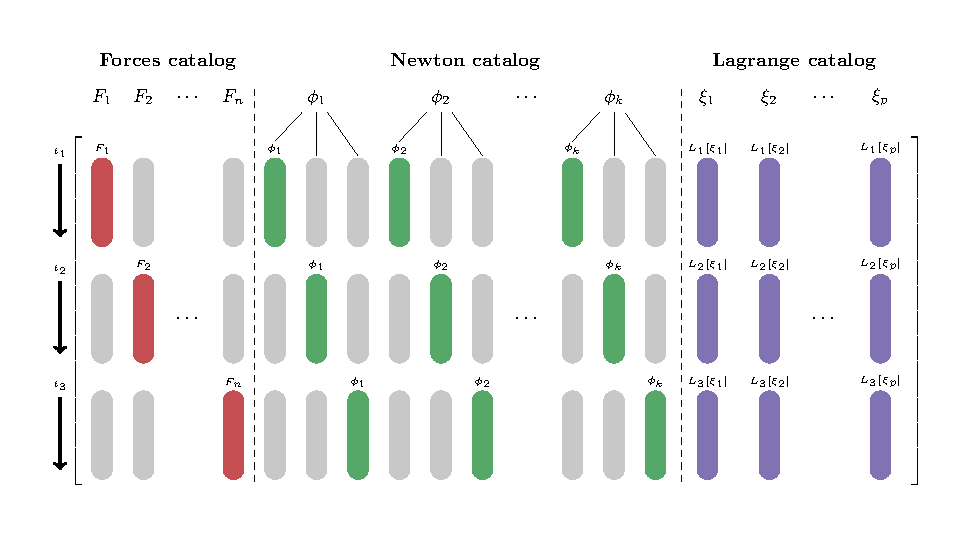
\includegraphics[width=1\textwidth]{solution_clustering} % for an image file named example_figure.*
	% Pick an appriopriate width for the size of the image

	% Captions go below figures
	\caption{\textbf{Unified Newton Lagrange matrix.}
		The combined matrix with Newton and Lagrange paradigm.}
	\label{fig:uni-sindy-matrix} % give each figure a logical label name
\end{figure}

\begin{figure} % Do not use \begin{figure*}
	\centering
	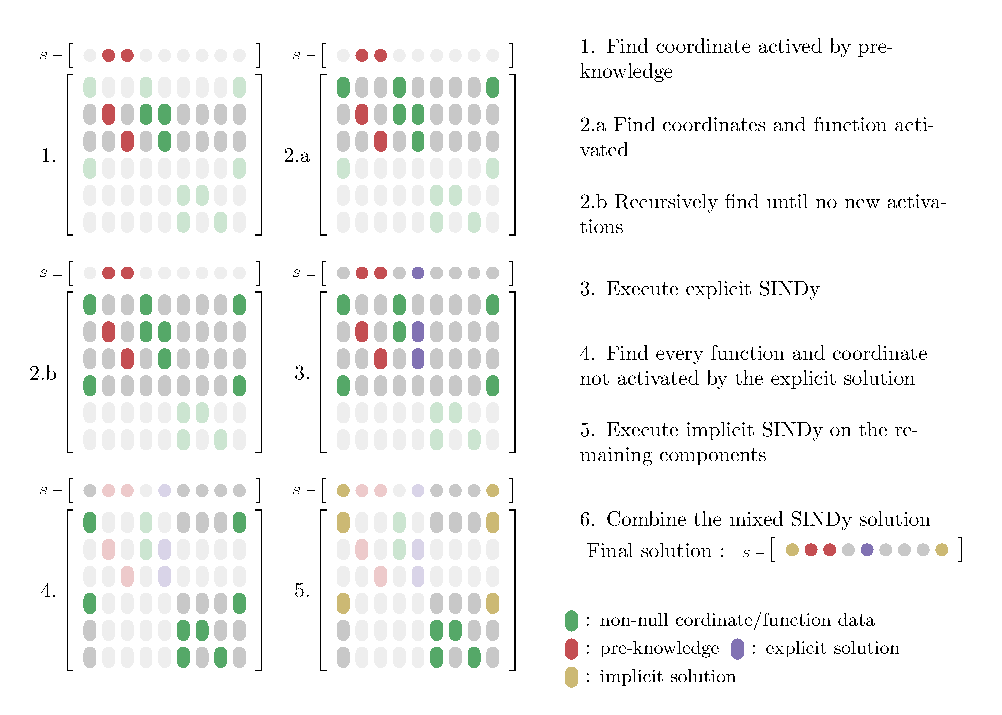
\includegraphics[width=1\textwidth]{mixed_algorithm} % for an image file named example_figure.*
	% Pick an appriopriate width for the size of the image

	% Captions go below figures
	\caption{\textbf{Mixed regression algorithm.}
		Algorithm developped to enable both explicit and implicit system in SINDy.}
	\label{fig:mixed_algorithm} % give each figure a logical label name
\end{figure}

% \begin{figure} % Do not use \begin{figure*}
% 	\centering
% 	\includegraphics[width=0.6\textwidth]{example_figure} % for an image file named example_figure.*
% 	% Pick an appriopriate width for the size of the image

% 	% Captions go below figures
% 	\caption{\textbf{All captions must start with a short bold sentence, acting as a title.}
% 		Follow the same style as main text figures.
% 		If the design is substantially the same as another figure, avoid repeating information
% 		e.g. say `Same as Figure~\ref{fig:example}, but for the control sample.'}
% 	\label{fig:sup_example} % give each figure a logical label name
% \end{figure}

%%%%%%%%%%%%%%%% SUPPLEMENTARY TABLES %%%%%%%%%%%%%%%

\begin{table} % Do not use \begin{table*}
	\centering
	% Captions go above tables
	\caption{\textbf{Catalog size for each paradigm.}
		Change in size are explained in data generation and processing. }
	\label{table:catalog_lenght} % give each table a logical label name

	\begin{tabular}{lccc} % four columns, alignment for each
		\\
		\hline
		System & Mixed solution & Newtonian & Lagrangian \\
		\hline
		Cartpole & 95 & 450 & 91 \\
		Double pendulum & 95 & 450 & 91 \\
		Cartpole double & 292 & 3360 & 283 \\
		\hline
	\end{tabular}
\end{table}



%%%%%%%%%%% CAPTIONS FOR OTHER SUPPLEMENTARY FILES %%%%%%%%%%

\clearpage % Clear all remaining figures and tables then start a new page

% \paragraph{Caption for Movie S1.}
% \textbf{All captions must start with a short bold sentence, acting as a title.}
% Then explain what is shown in the supplementary video file.
% Give as much detail as you would for a figure e.g. explain axes, color maps etc.
% If the video is an animated equivalent of one of the static figures, state e.g.
% `Animated version of Figure~\ref{fig:example}.'

% \paragraph{Caption for Data S1.}
% \textbf{All captions must start with a short bold sentence, acting as a title.}
% Then explain what is included in the supplementary data file.
% Give as much detail as you would for a table e.g. explain the meaning of every column,
% units used, any special notation etc.


%%%%%%%%%%%%%%%% SUPPLEMENTARY REFERENCES %%%%%%%%%%%%%%%

% Do NOT include a reference list in the supplement.
% All references must be in a single list at the end of the main text.
% The copyeditors will ensure that the correct reference list appears with each version of the paper
% (print, HTML, PDF, mobile app, metadata for bibliographic databases etc.)

\end{document}
% End of science_template.tex